\documentclass[ngerman]{scrartcl} %lädt die Dokumentklasse
                                %Artikel von Koma-Skript, als Option
                                %übergebe ich, dass ich die Trennung
                                %nach neuer deutscher Rechtschreibung
                                %wünsche
\usepackage[ngerman]{babel}
\usepackage[utf8]{inputenc}
\usepackage{color}
\usepackage[T1]{fontenc}
\usepackage[pdfborder={0 0 0}]{hyperref}
\usepackage[a4paper,lmargin={2,5cm},rmargin={2,5cm},tmargin={2.5cm},bmargin = {2.5cm}]{geometry}
\usepackage[onehalfspacing]{setspace}
\usepackage{amssymb}
\usepackage{graphicx}
\usepackage{amsthm}
\usepackage{graphicx}
\usepackage{url} 
\usepackage{listings}
\usepackage{acronym} 
\usepackage{tabularx}
\usepackage{float}

% Macht für jede Section eine neue Seite
\usepackage{titlesec}
\newcommand{\sectionbreak}{\clearpage}

\begin{document}

\thispagestyle{empty}
\begin{figure}[!htb]
\minipage{0.32\textwidth}%
  
\includegraphics[width=\linewidth]{DHBW-Logo.png}
  \label{fig:awesome_image3}
\endminipage
\end{figure}

\begin{center}
\vfill
{\Large Amazon Dash selbstgebaut}
\vfill
\textbf{STUDIENARBEIT}
\vfill

des Studienganges Angewandte Informatik\\
\vspace{12pt}
an der Dualen Hochschule Baden-Württemberg Stuttgart
\vfill

von\\
\vspace{12pt}
Tobias Fürtjes, Lennart Roger Jerker Gustafsson, Kai Fabian Oswald
\vfill

\today
\vfill

\begin{tabular}{ll}
Bearbeitungszeitraum & 33 Wochen \\
Matrikelnummern, Kurs & 7747179 (Fürtjes), 5335024 (Gustafsson), 7805276 (Oswald) TINF-14C \\
Betreuer & Martin Kissel \\
\end{tabular}

\end{center}   

\pagenumbering{roman}
\section*{Ehrenwörtliche Erklärung}

Erklärung\\
\newline
gemäß § 5 (3) der „Studien- und Prüfungsordnung DHBW Technik“\\
vom 22. September 2011.\\
\newline
Ich habe die vorliegende Arbeit selbstständig verfasst und keine anderen\\
als die angegebenen Quellen und Hilfsmittel verwendet.\\

\begin{flushleft}
\begin{tabularx}{\textwidth}{XX}
\noindent\rule{6cm}{0.4pt} & \noindent\rule{6cm}{0.4pt} \\
(Datum, Ort) & (Unterschrift) \\
\noindent\rule{6cm}{0.4pt} & \noindent\rule{6cm}{0.4pt} \\
(Datum, Ort) & (Unterschrift) \\
\noindent\rule{6cm}{0.4pt} & \noindent\rule{6cm}{0.4pt} \\
(Datum, Ort) & (Unterschrift) \\
\end{tabularx}
\end{flushleft}
\newpage

\addcontentsline{toc}{section}{Inhaltsverzeichnis}
\tableofcontents

\addcontentsline{toc}{section}{Abbildungsverzeichnis}
\listoffigures

\addcontentsline{toc}{section}{Tabellenverzeichnis}
\listoftables 
 
\section*{Abkürzungsverzeichnis}
\addcontentsline{toc}{section}{Abkürzungsverzeichnis}
\label{sec:Abkürzungsverzeichnis}
\begin{acronym}[Bash]
 \acro{API} {Application Programming Interface}
 \acro{ARP} {Address Resolution Protocol}
 \acro{GPIO} {General Purpose Input/Output}
 \acro{IoT} {Internet of Things}
 \acro{IDE} {Integrated Development Environment}
 \acro{IP} {Internet Protokoll}
 \acro{JSON} {JavaScript Object Notation}
 \acro{ORM} {Object Relation Mapping}
 \acro{OSI} {Open Systems Interconnection}
 \acro{PHP} {PHP: Hypertext Preprocessor}
 \acro{REST} {Representational State Transfer}
 \acro{TCP} {Transmission Control Protocol}
 \acro{UDP}{User Datagram Protocol}
 \end{acronym}


\section{Einleitung}        
\label{sec:Einleitung-1}   
\pagenumbering{arabic}
In den letzten Jahren konnten aufgrund technologischer Entwicklungen immer mehr Geräte entwickelt werden, die in den verschiedensten Bereichen des täglichen Lebens eingesetzt werden. Diese Entwicklungen betreffen dabei meist die Leistungsfähigkeit, Konnektivität oder Größe der Geräte, sodass sie in immer mehr und unterschiedlicheren Bereichen eingesetzt werden können. Ein Begriff der in den letzten Jahren für dieses Phänomen immer häufiger genutzt wurde, ist das ``\ac{IoT}'' zu deutsch ``Das Internet der Dinge''. Mit dem \ac{IoT} wird beschrieben, dass immer mehr Geräte mit dem Internet verbunden sind und Daten austauschen. Im Rahmen dieser Entwicklung sind verschiedenste Nutzungsszenarien umgesetzt worden, die das tägliche Leben erleichtern oder automatisieren sollen. Diese Studienarbeit wird sich im folgenden mit einem speziellen Szenario befassen, welches unter anderem durch den Onlinehändler Amazon umgesetzt wurde.

Das Szenario umfasst sogenannte ``Amazon Dash Buttons''. Diese Buttons sind kleine Geräte, welche an unterschiedlichen Stellen in der Wohnung des Kundens angebracht werden können und über einen Druckknopf verfügen. Nach einer Konfiguration durch den Benutzer kann mithilfe eines Drucks auf den Sensor ein zuvor ausgewähltes Produkt bestellt werden. Ein Beispiel wäre das nachbestellen von Waschpulver. So könnte der Button an der Waschmaschine befestigt sein und bei einem geringen Vorrat an Waschpulver wird der Button betätigt und das ausgewählte Waschpulver innerhalb der nächsten Tage geliefert. So entfällt für den Nutzer der händische Bestellvorgang, da dieser automatisch durch den Button und Amazon durchgeführt wird. Dieses Beispiel lässt sich natürlich auf verschiedene andere Möglichkeiten übertragen, so könnten auch Dinge, wie Kaffee, Zahnpasta, Tierfutter, Getränke oder ähnliches nachbestellt werden. Dem Nutzer wird eine Vereinfachung des Kaufprozesses versprochen und der Händler bindet den Kunden stärker an sich, da der Button direkt bei Amazon bestellt. 
Die Studienarbeit setzt sich zum Ziel eine Untersuchung des Amazonproduktes durchzuführen und die Machbarkeit und Umsetzung einer offeneren Lösung zu prüfen. 

    

\section{Aufgabenstellung}
\label{sec:Aufgabenstellung-1}
Wie bereits in der \nameref{sec:Einleitung-1} erwähnt, soll sich diese Studienarbeit mit der Untersuchung des Amazon Dash Buttons beschäftigen und eine Alternative entwickeln. Da bereits während der Recherche vor Projektbeginn herausgefunden werden konnte, dass der Button in der Standardkonfiguration nur mit den Services von Amazon zusammenarbeiten kann, soll eine offenere Lösung entwickelt werden. Mit einer offeneren Lösung wird im Rahmen dieser Studienarbeit eine Möglichkeit definiert, die dem Kunden einen ähnlichen Funktionsumfang anbietet. Ein grundlegender Unterschied ist jedoch im Bestellprozess vorhanden. Während die Lösung von Amazon eine direkte Bestellung bei Amazon auslöst, soll die offenere Lösung eine Einkaufsliste mit Produkten erstellen. 

Der Nutzer soll dann über ein Webfrontend die Möglichkeit haben den Einkaufszettel zu betrachten und dann die entsprechenden Produkte bei seinem bevorzugten Händler zu bestellen. So kann es auch möglich sein, dass auch Produkte geführt werden, die der Nutzer nicht online bestellen kann. Der Vorteil bei dieser Lösung liegt darin, dass der Nutzer nicht an einen Händler und dessen Preise gebunden ist, sondern die Preise vergleichen und einen entsprechenden Händler, der seinen persönlichen Kriterien entspricht, wählen kann. 
Im Rahmen dieses Ziels müssen verschiedene Komponenten entwickelt werden, die im Rahmen der Lösung zusammenarbeiten. Diese Komponenten lassen sich unter folgenden Kategorien zusammenfassen:
\begin{itemize}
\item Entwicklung von Buttons 
\item Entwicklung eines Frontends zur Nutzerinteraktion
\item Entwicklung eines Backends zur Verarbeitung von Frontendeingaben und der Eingabe von Buttons 
\end{itemize}
Die Entwicklung von Buttons lässt sich dabei in zwei Teile aufteilen. Zum einem soll der Amazon Dash Button betrachtet und analysiert werden. In diesem Rahmen soll sowohl die Einrichtung und Konfiguration als auch die Kommunikation untersucht werden. In Folge dessen soll weiterhin geprüft werden, ob der Button auch für die offene Lösung genutzt werden kann und dabei kein Produkt bei Amazon bestellt. Weiterhin sollen mithilfe von Mikrokontrollern eigene Buttons entwickelt werden, die ebenfalls ein Signal an den entsprechenden Empfänger absenden können. Bei den Buttons steht die Funktionalität und die Prüfung der Machbarkeit des Projektes im Vordergrund. Die Gestaltung der Buttons spielt keine priorisierte Rolle. 


Weiterhin muss ein Frontend entwickelt werden, welches die Nutzerinteraktion ermöglicht. Das Frontend soll zur Übersicht der Einkaufsliste genutzt werden, aber auch die Verwaltung der Buttons und andere anfallende Verwaltungsfunktionen sollen ermöglicht werden. 
Um eine Kommunikation zwischen Frontend und den Buttons zu gewährleisten, muss ein Backend entwickelt werden, welches über Schnittstellen die Kommunikation gewährleistet und die Eingaben entsprechend verarbeitet. 
Als Ergebnis des Projektes soll möglichst ein eigener Button entstanden sein, der mithilfe des Backends und Frontends dem Nutzer ermöglicht einen ähnlichen, aber offeneren Prozess, wie bei Amazon, zu nutzen. Weiterhin soll zumindest der Amazon Dash Button untersucht worden sein und wenn möglich miteingebunden sein. Abschließend soll ein Fazit gezogen werden, inwiefern das Projekt umsetzbar ist. 

\section{Theorie}        
\label{sec:Theorie-1}  
Im Rahmen dieser Arbeit wurden verschiedene Technologien und Prinzipien eingesetzt. Auf diese soll in den folgenden Unterkapiteln eingegangen werden, damit eine theoretische Grundlage vorhanden ist. 

\subsection{\ac{UDP}}
\label{sec:UDP-1}

\ac{UDP} steht für ``User-Datagram-Protocol'' und ist ein verbindungsloses Transportprotokoll. Im \ac{OSI}-7-Schichten Modell arbeitet es auf der Transportebene und ist für die Zustellung von Netzwerkpaketen von einem Sender zu einem Empfänger zuständig. Im Vergleich zum Transportprotokoll \ac{TCP}, welches verbindungsorientiert arbeitet, ist es wesentlich einfacher zu verarbeiten, da beispielsweise der Header bei den einzelnen Datenpaketen wesentlich kleiner ist. Allgemein ist es sehr minimal gehalten und dadurch sehr einfach zu implementieren und für sehr einfache Anwendungszwecke geeignet. Allerdings ist auch zu erwähnen, dass es keine Empfangsbestätigung gibt und die Daten nach dem Absenden nicht weiter kontrolliert werden. Somit können die Daten auch im Netzwerk verloren gehen und es wird nicht bemerkt. \\
Der einfache Header des \ac{UDP} Protokolls besteht nur aus vier Attributen. Diese jeweils 16 Bit großen Felder enthalten den Quellport, den Zielport, die Checksumme zur Überprüfung des Inhalts und die Länge des gesamten Pakets. Insgesamt ist der Header somit 8 Byte groß. (vgl. \cite{ElektronikKompendium.}\cite{.}\cite{.23.02.2016})
 

\subsection{\ac{TCP}}
\label{sec:TCP-1}

\ac{TCP} ist ein verbindungsorientiertes Protokoll, dass im \ac{OSI}-7-Schichten Modell auf der vierten Ebene (Transport) einzuordnen ist. Im sogenannten \ac{TCP}/\ac{IP} Protokollstapel ist es in der dritten von vier Schichten zu finden. Bei einer Übertragung von Daten über \ac{TCP} übergibt die genutzte Anwendung den Datenstrom an das Protokoll und empfängt ihn auch wieder von dort. Für die Übertragung ist dementsprechend \ac{TCP} zuständig. 
Die Hauptaufgaben des Protokolls sind daher die Aufteilung und die Zusammensetzung der Daten von entsprechend vielen Paketen (Segmentierung), das Management der Verbindung und ein entsprechendes Fehlerhandling, welches das korrekte Empfangen von Paketen überwacht. Das Fehlerhandling nutzt eine positive Bestätigung aller Pakete. Dies bedeutet, dass nur nicht vorhandene Pakete erneut angefragt werden, ansonsten davon ausgegangen wird, dass die Daten beim Empfänger angekommen sind. Diese Technologie sorgt dafür, dass die Daten auf jeden Fall ankommen, sofern die Verbindung nicht gestört wird (vgl. \cite{.c}\cite{.22.11.2016}).

Der Header eines \ac{TCP} Pakets besteht aus 20 Bytes, jedoch kann dieser auch noch erweitert werden, sodass noch einige zusätzliche Bytes in den Header geschrieben werden. Zu den zwingend notwendigen Daten gehört unter anderem der Port auf dem das Paket empfangen wird und der Port über den das Paket gesendet wird. Zudem wird die Nummer im aktuellen Paketstrom benötigt. Zudem wird eine Prüfsumme und Quittierungsnummer mitgegeben, welche zur Kontrolle und Bestätigung genutzt werden (vgl \cite{.c}).


\subsection{\ac{ARP}}
\label{sec:ARP-1}

Das \ac{ARP} Protrokoll ist ein Protrokoll, dass auf der zweiten Ebene (Sicherungsebene) des OSI Modells wiederzufinden ist. Mithilfe von \ac{ARP} werden in einem Netzwerk die vergebenen \ac{IP} Adressen in MAC Adressen beziehungsweise Hardwareadressen ungewandelt. Dieser Prozess ist notwendig, da innerhalb eines lokalen Netzwerkes die Netzwerkpakete über diese MAC Adressen an die entsprechenden Empfänger geleitet werden. Da zuvor die Kommunikation über \ac{IP} lief, muss diese Umwandlung durchgeführt werden. 
Diese Unwandlung wird mithilfe von \ac{ARP} realisiert. Sobald ein Gerät einem Netzwerk beitritt, wird ein \ac{ARP} Request an die Adresse ``FF-FF-FF-FF-FF-FF'' geschickt. Diese Adresse ist ein sogenannter Broadcast, der diesen Request an alle Geräte im Netzwerk schickt. Dieser Request wird vom Router so verarbeitet, indem er der, im Request mitgesendeten, MAC Adresse des Geräts eine \ac{IP} Adresse zuordnet, die für das IP Protrokoll verwendet werden kann. Nach diesem erfolgreichen Mapping einer \ac{MAC} Adresse im Netzwerk auf eine \ac{IP} Adresse, kann die weitere Kommunikation beispielsweise über das Internet Protrokoll oder andere Protrokolle genutzt werden. Aufgrund des hinterlegten Mappings weiß der Router nun, zu welcher \ac{MAC} Adresse er die entsprechenden Pakete mit einer bestimmten \ac{IP} Adresse weiterleiten muss. (vgl. \cite{.r}\cite{.q})

\subsection{Webserver: Nginx}
\label{sec:WebserverNginx-1} 

Nginx bestitzt einen Marktanteil von ca. 20 Prozent aller Webserver und ist somit auf Rang 2 der Webserver für aktive Webseiten hinter Apache und vor Microsoft und Google\cite{.k}. In dieser Studienarbeit haben wir uns für nginx entschieden, da ein hoher Wert auf eine flexible Konfiguration und schnelle Serverantworten gelegt wird. Folgend werden die Hauptfeatures von Nginx genauer beschrieben.

\subsubsection{Allgemein}
\label{sec:NginxAllgemein}
Nginx ist ein HTTP und Reverse-Proxy Server, ein Mail-Proxy Server und ein allgemeiner TCP/UDP Proxy-Server. Somit hat Nginx eine hohe Nutzungsbreite.

\subsubsection{Features}
\label{sec:NginxFeatures}
Die von Nginx unterstützten Features werden im Folgenden gegliedert nach den jeweiligen Einsatzgebeiten vorgestellt.\cite{.14.03.2017}


\subsubsection{Basic HTTP}
\label{sec:NginxBasicHTTP}
Nginx unterstützt die Bereitstellung von statischen Dateien. Durch die modulare Architektur ist Nginx für viele Zwecke einsetzbar und bleibt dabei übersichtlich. HTTP/2 wird unterstützt, was die Übertragung beschleunigt und optimiert. Das Rewrite Modul ermöglicht die Änderungen von URIs anhand von regulären Ausdrücken. Dies trägt auch zur Suchmaschinenoptimierung bei und ermöglicht das Erstellen von lesbaren URIs. Die Zugriffskontrolle kann anhand von IP-Adressen oder Passwörtern erfolgen. Anhand der IP-Adresse können zudem Informationen zu Geolocation gewonnen werden. SSL und TLS SNI wird natürlich auch unterstützt.

\subsubsection{Mail Proxy-Server}
\label{sec:NginxMail Proxy-Server}
Die Authentifizierung kann über einen externen HTTP Server durchgeführt werden, welcher dann nach erfolgreicher Authentifizierung zu einem internen SMTP-Server weiterleitet. Somit muss man sich nicht direkt am Mail-Server authentifizieren. Zudem wird SSL, STARTTLS und STLS unterstützt.

\subsubsection{TCP/UDP Proxy-Server}
\label{sec:NginxTCP/UDP Proxy-Server}
Allgemeine Proxy-Features von TCP und UDP sind vorhanden. Des Weiteren wird SSL und TLS SNI auch für TCP unterstützt.
Um vor Überlastungen zu schützen können Verbindungen, die von derselben Adresse kommen begrenzt werden. Zugriffskontrolle geschieht anhand der Benutzeradresse. Es werden zudem auch Features unterstützt, die den Lastausgleich und die Fehlertoleranz verbessern.


\subsubsection{Architektur und Skalierbarkeit}
\label{sec:NginxArchitektur und Skalierbarkeit}
Nginx ist so aufgebaut, dass es einen Master und mehrere Worker-Prozesse gibt. Die Worker brauchen dabei keinerlei spezielle Berechtigungen, so muss nur dem Master entsprechende Berechtigungen gewährt werden. Des Weiteren ist eine flexible Konfiguration möglich. Die Nginx Konfiguration für diese Studienarbeit befindet sich im Anhang unter Abschnitt \ref {sec:NginxKonfiguration}.

 
\subsection{Arduino}
\label{sec:Arduino-1} 

Die Bezeichnung Arduino steht für eine Technologie, die sowohl aus einer Hardwarekomponente als auch aus einer Softwarekomponente besteht. Zudem gibt es zwei Unternehmen, die in ihrem Namen den Begriff Arduino tragen und in Zusammenhang mit der Technologie stehen. Zum einem gibt es die Arduino LLC, die die Gruppe der Gründer der Plattform bezeichnet. Des Weiteren gibt es die Arduino S.r.l., das die Firma bezeichnet, die anfangs allein die Arduinoboards produzierte und dann auch verkaufte. Die Arduinoplattform wurde ursprünglich entwickelt, um Anfängern den Einstieg in die Mikrokontrollerprogrammierung zu vereinfachen. 

Grundsätzlich besteht die sogenannte Arduinoplattform aber sowohl aus der Hardware als auch der Software. Die Hardware umfasst mittlerweile verschiedene Mikrokontroller beziehungsweise Einplatinencomputer, welche für verschiedene Anwendungszwecke genutzt werden können. Die entsprechende Nutzung wird mithilfe der richtigen Programmierung erreicht. Dafür kann der Softwareteil der Lösung genutzt werden, welches aus einer \ac{IDE}  besteht und das Schreiben von Programmen vereinfacht. Zudem wird über diese \ac{IDE} auch die Kommunikation mit dem Mikrokontroller realisiert. Diese Entwicklungsumgebung eignet sich für diverse Mikrokontroller, sofern entsprechende Treiber verfügbar sind, können auch Boards genutzt werden, die nicht direkt mit Arduino zusammenhängen. Zudem kann in verschiedenen Programmiersprachen entwickelt werden, beispielsweise C oder C++. (vgl. \cite{.h,.f,.e,.i,.g,online.})
Die komplette Plattform ist open source, auch wenn die Hardware natürlich erworben werden muss. 



\subsection{Python}
\label{sec:Python-1}

Python ist eine objektorientierte Programmiersprache und wurde 1991 in der ersten Version von Guido van Rossum veröffentlicht (vgl. \cite{.05.03.2017}). Zu den technischen Merkmalen gehört unter anderem die Unterstützung von Paketen beziehungsweise Bibliotheken, die die entsprechend benötigten Funktionen laden, sofern sie in das Projekt eingebunden werden. 

Außerdem ist eines der Merkmale die Einrückung. Python nutzt nicht, im Gegensatz zu anderen Programmiersprachen, bestimmte Klammern oder andere Symbole um den Code zu strukturieren, sondern verwendet stattdessen die Einrückung von den entsprechenden Zeilen Code. Das bedeutet, dass zum Beispiel nach einem Methodenkopf keine geschweifte Klammer oder ähnliches verwendet wird, sondern die nächste Zeile wird um beispielsweise vier Leerzeichen eingerückt. Das Methodenende wird dadurch definiert, dass ein anderer Codeabschnitt wieder auf der gleichen Einrückungsstufe steht, wie der Methodenkopf (vgl. \cite{.19.08.2013}\cite{.10.03.2017b}). 
Zudem ist Python eine dynamische Programmiersprache und es ist möglich Python als Skriptsprache zu verwenden und Skripte zu schreiben, die mithilfe des Interpreters ausgeführt werden. Durch die Möglichkeit Python auch auf Linux zu verwenden, können diese Skripte auch entsprechend unter Linux verwendet werden.

Python kann für verschiedene Anwendungszwecke genutzt werden, es gibt zum Beispiel verschiedene Möglichkeiten der Stringverarbeitung, die Möglichkeit mit verschiedenen Internetprotokollen zu arbeiten, beispielsweise \ac{HTTP}, \ac{FTP} oder \ac{SMTP} aber auch auf Interfaces des Betriebssystems zuzugreifen, um beispielsweise mit Sockets (z.B. \ac{TCP}/\ac{IP} Sockets) zu arbeiten. Neben diesen Funktionen, die durch die Standardbibliotheken abgedeckt werden, gibt es auch noch weitere Pakete, die weitere Bibliotheken mit Funktionen hinzufügen. So gibt es zum Beispiel die Möglichkeit das Paket BeautifulSoup oder Requests hinzuzufügen. Letzteres bietet zum Beispiel viele Möglichkeiten mit dem \ac{HTTP} Protokoll zu arbeiten (vgl \cite{.m}\cite{.l}\cite{.05.03.2017}). 




\subsection{MySQL}
\label{sec:MySQL-1}

MySQL ist ein relationales Datenbankverwaltungssystem, welches in einer Open Source als auch einer kommerziellen Version verfügbar ist. Es basiert auf der Datenbanksprache \ac{SQL} und wird häufig in Kombination mit \ac{PHP} verwendet. Die kommerzielle Version wird von der Firma MySQL AB entwickelt, die wiederrum im Jahr 2008 von Sun übernommen wurde. Da Sun durch Oracle übernommen wurde, gehört nun auch die Firma MySQL AB zu Oracle.  Zudem ist es eines der am häufigsten genutzten Datenbanksysteme. (vgl. \cite{.q}\cite{Horn.12.03.2017})
 
\subsection{Frontendtechnologien}
\label{sec:Frontendtechnologien-1}

Um eine dynamische und nutzerfreundliche Oberfläche zu schaffen wurden Frameworks benutzt. 
Für die Gestaltung der einzelnen Komponenten wurde Bootstrap verwendet, welches für alle wichtigen Komponenten bereits vorgefertigte Styles enthält.
Dies beschleunigt den Prozess der Gestaltung der Oberfläche enorm, da nicht jede verwendete Komponente manuell anhand von \ac{CSS} gestaltet werden muss. 
Die verwendete Bootstrap Version ist Version 3.

Bootstrap ermöglicht es ohne großen Aufwand responsive Webseiten zu gestalten. 
Dabei soll während der Entwicklung auf das mobile-first Prinzip Wert gelegt werden. 
Dieses Prinzip besagt, dass zuerst die Seite für mobile Endgeräte optimiert wird und anschließend erst auf größere Monitore beziehungsweise Auflösungen geachtet werden soll. 
Weltweit liegt der Anteil aller Website-Aufrufe von mobilen Endgeräten bei fast 50\% (vgl. \cite{.stat-mobile}). 

Für die Dynamik sorgt das JavaScript-Framework Vue. Mit Vue vergleichbare Frameworks sind React und Angular. Vue wird verwendet, da es eine große Community hat, eine gute Dokumentation vorweist, sowie eines der besten Frameworks performancetechnisch ist (vgl. \cite{.vue-react-angular}).
Frontend Frameworks, wie auch Vue, bieten die Funktionalität Komponenten zu erstellen und diese beliebig zu verwenden. 
Des Weiteren erhöhen sie, vorausgesetzt sie werden richtig eingesetzt, die Nutzererfahrung, da nicht bei jeder Aktion die komplette Seite neu geladen werden muss.

Folgend wird etwas genauer auf das Vue-Framework eingegangen. 
Komponenten sind das Herzstück von Vue. Sie besitzen jeweils genau ein Template, welches in \ac{HTML} definiert ist. 
Des Weiteren haben Komponenten Daten, die durch data-binding automatisiert geändert werden. 
Beispielsweise kann man eine Variable an ein Input-Element binden und wenn dieses einen anderen Wert annimmt wird auch automatisch die Variable angepasst. 
Daten können dabei direkt bei der Initialisierung der Komponente oder zu einem späteren Zeitpunkt geladen werden.
Dadurch wird die initiale Ladezeit der Seite deutlich verringert, da die Daten asynchron geladen werden.

 
\newpage
 
\subsection{\ac{REST}}        
\label{sec:REST-1}  

\subsubsection{\ac{REST} Allgemein}
\label{sec:RESTAllgemein}

Im Folgenden soll die Technologie \ac{REST} vorgestellt werden.
Zunächst wird \ac{REST} etwas genauer anhand von Beispielen erläutert.
Anschließend werden die Vor- und Nachteile dargestellt, sowie die Kernpunkte erläutert.

\subsubsection{\ac{REST} Beispiel}
\label{sec:RESTBeispiel}

Um Daten von einer \ac{REST}-Schnittstelle zu bekommen, werden die \ac{HTTP}-Methoden in Verbindung mit einer entsprechenden \ac{URI} verwendet. Im Folgenden wird dies anhand einiger Beispiele gezeigt:

GET /resources/
Liefert eine Liste aller Ressourcen.

GET /resources/4
Liefert die Ressource mit ID = 4.

POST /resources/
Legt eine neue Ressource an.

PUT /resources/4
Aktualisiert die Ressource mit ID = 4.

DELETE /resources/4
Löscht die Ressource mit ID = 4.

Einen tieferen Einblick, wann und wie die Methoden genutzt werden, wird in Abschnitt \ref{sec:RESTHTTP} gegeben.

\subsubsection{Ressourcen}
\label{sec:RESTRessourcen}

Im Folgenden werden Datensätze als Ressourcen bezeichnet. Dabei kann man die Ressourcen weiter unterteilen:

–	Primärressourcen: Unter Primärressourcen fallen komplette, vollständige Ressourcen

–	Subressourcen: Subressourcen sind Teile von Primärressourcen

–	Listen: Eine Liste umfasst eine Menge von Ressourcen

–	Filter: Anwendung von Filterkriterien auf Listen

–	Paginierung: begrenzte Datenmenge

–	Projektionen: Teil der Informationen einer Primärressource

–	Aggregationen: Zusammenfassung mehrerer Ressourcen

\subsubsection{Merkmale}
\label{sec:RESTMerkmale}

Die Kommunikation erfolgt auf Abruf. Der Client ist aktiv und fordert vom passiven Server eine Repräsentation an, bzw. modifiziert eine Ressource. Ressourcen, die Objekte der Anwendung, besitzen eine ihnen zugeordnete \ac{URI}, mit der sie adressiert werden können. Die Repräsentation einer Ressource kann als Dokument vom Client angefordert werden. Repräsentationen können auf weitere Ressourcen verweisen, die ihrerseits wieder Repräsentationen liefern, die wiederum auf Ressourcen verweisen können. Der Server verfolgt keinen Clientstatus. Jede Anfrage an den Server muss alle Informationen beinhalten, die zum Interpretieren der Anfrage notwendig sind. Caches werden unterstützt. Der Server kann seine Antwort als cache-fähig oder nicht cache-fähig kennzeichnen.

Repräsentationen:

Um die Ressourcen darzustellen, werden in REST mehrere Repräsentationen der Ressourcen genutzt. Dies entsteht aus der Intention heraus, dass aufgrund der unterschiedlichen Repräsentationen unterschiedliche Anforderungen der Clients bedient werden können. So kann zum Beispiel die \ac{HTML} Repräsentation für einen Webbrowser genutzt werden, während eine \ac{JSON} Repräsentation für eine Clientapplikation genutzt wird.

\subsubsection{HTTP}
\label{sec:RESTHTTP}


Um auf eine Ressource zuzugreifen wird das \ac{HTTP}-Protokoll verwendet. Je nachdem, welche Verwendung die Ressourcen finden, werden geeignete \ac{HTTP}-Methoden verwendet. Die häufigsten Verwendeten Methoden sind dabei GET, POST, PUT und DELETE. Per GET werden Daten geladen; POST hat mehrere Einsatzgebiete. Häufig wird dadurch eine neuer Datensatz angelegt, oder mehrere Datensätzen aktualisiert. PUT aktualisiert einen bestimmten Datensatz und DELETE löscht einen Datensatz. Dabei müssen sinnvolle Statuscodes zurückgegeben werden. Zusätzlich gibt es noch die Methoden PATCH, HEAD und OPTIONS. Auf diese wird jedoch nicht weiter eingegangen, da diese eine vergleichsweise geringe Bedeutung bei einer REST-Schnittstelle haben. Bei der Implementierung ist unbedingt zu beachten die Methoden idempotent zu gestalten, d.h. Ein mehrmaliges Aufrufen derselben Methode wirkt sich nicht anders aus, als ein einmaliger Aufruf. Einzige Ausnahme dabei ist die POST-Methode. Das Prinzip von \ac{REST} ist, Ressourcen von einem Zustand in den nächsten Zustand zu überführen.

\subsubsection{Statuscodes}
\label{sec:RESTStatuscodes}

Folgende Tabelle zeigt die allgemeine Bedeutung der unterschiedlichen Statuscodes

\begin{table}[!h]
	\begin{tabular}{ | l | l | }
		\hline
		Statuscode & Bedeutung \\ \hline
		1xx & Informationen \\ \hline
		2xx & Erfolgreiche Operationen \\ \hline
		3xx & Umleitung \\ \hline
		4xx & Client-Fehler \\ \hline
		5xx & Server-Fehler \\ \hline
	\end{tabular}
	\caption{Statuscodes}
\end{table}


\subsubsection{URI-Design}
\label{sec:RESTURI-Design}

Eine \ac{URL} lokalisiert eine Ressource, wobei eine \ac{URI} sie identifiziert. Lokalisierung kann dabei auch zur Identifizierung führen.
Eine \ac{URL} ist also immer eine \ac{URI}. Im Umkehrschluss kann eine \ac{URI} eine \ac{URL} sein, muss es
aber nicht.

Möchte man \ac{REST} in einem Satz definieren, dann ergibt sich: „Eine eigene URI für jedes Informationselement.“ (vgl. \cite{.j}\cite{Tilkov.2015b})

An diesem Satz sollte man sich auch beim \ac{URI}-Design halten. Ressourcen können so durch
ihre \ac{URI} eindeutig identifiziert werden. Dabei sollen diese so konstruiert werden, dass man
bereits aus der \ac{URI} alleine lesen kann, was für eine Ressource dahinter steckt. Eine \ac{URI} zeigt
auf eine Ressource, aber diese kann über mehrere \ac{URI}s angesprochen werden.
Die verschiedenen Ressourcenarten können auf folgende \ac{URI}-Strukturen abgebildet werden (vgl. Kapitel \ref{sec:RESTRessourcen}): 

–	Liste: /resources/:	Man bekommt mehrere Ressourcen gleicher Art

–	Primärressource: /resources/1:	Man bekommt genau eine unabhängige Ressource

–	Sekundärressource: /resources/subresources/1:	Man bekommt genau eine von einer anderen Ressource abhängige Ressource

–	Filter: /resources?name=a oder /resources/name=a : Man bekommt mehrere Ressourcen gleicher Art, die mit bestimmten Parametern gefiltert werden.

\subsubsection{HATEOAS}
\label{sec:RESTHATEOAS}

HATEOAS ist ein wichtiges Prinzip, welches von vielen selbsternannten \ac{REST}-Schnittstellen
nicht implementiert wird. Dieses Akronym beschreibt, dass die Schnittstelle über Hypertext
beziehungsweise Hypermedia angetrieben wird. Genauer gesagt, sollen durch den Aufruf
der Haupt-URI alle Funktionalitäten als Hyperlinks unter Angabe der jeweiligen Beziehung
zugreifbar sein. Die Schnittstelle dokumentiert sich sozusagen selbst.
In seiner im Jahre 2000 verfassten Dissertation “Architectural Styles and the Design of
Network-based Software Architectures”, definiert Roy Fielding die \ac{REST}-Architektur. Dabei
geht er unter anderem auf Ressourcen und \ac{HTTP} ein. Als wichtigen Punkt sieht Fielding
jedoch auch die Verwendung von Hypermedia und die Verlinkung zwischen verwandten Ressourcen.
In 2008 verdeutlicht Fielding anhand eines Blogeintrags seinen Standpunkt zu RESTful API’s...
“If the engine of application state (and hence the API) is not being driven by hypertext, then
it cannot be RESTful and cannot be a REST API. Period. Is there some broken manual
somewhere that needs to be fixed?” – \cite{.19.03.2017}

Damit will er sagen, dass Schnittstellen, welche nicht über Hypertext gesteuert werden, auch
keine \ac{REST}-Schnittstellen sind, sondern ganz normale RPC-Schnittstellen.
Um dieses Prinzip zu verdeutlichen wird anhand Abbildung 3 das Richardson Maturity Model
veranschaulicht.
 
\begin{figure}[!htb]
	\centering
	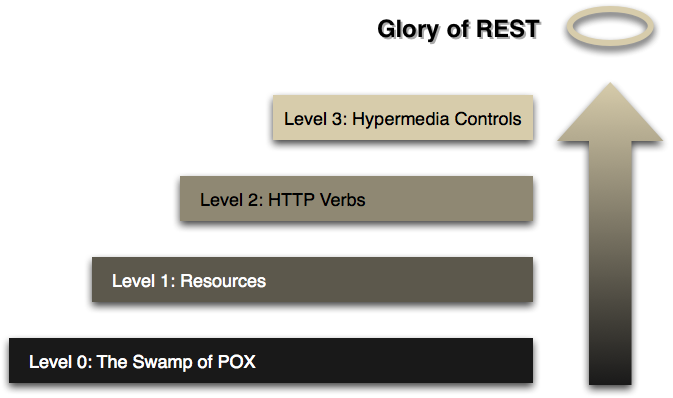
\includegraphics[scale=0.5]{hateoas.png}
	\caption[Richardson Maturity Model]{Richardson Maturity Model,\\ Quelle: https://martinfowler.com/articles/images/richardsonMaturityModel/ overview.png}
\end{figure}
 


Das Richardson Maturity Model unterteilt die \ac{REST}-Architektur in vier Stufen. Eine echte
\ac{REST}-Schnittstelle implementiert dabei alle vier Stufen. Doch gerade die letzte Stufe wird oft
nicht implementiert, da sie eine gewisse Komplexität birgt.

LEVEL 0 sagt lediglich aus, dass \ac{HTTP} als Transportprotokoll für RPC-Aufrufe genutzt wird.
Die Kommunikation findet über eine einzige \ac{URI} statt.

LEVEL 1 sagt aus, dass jede Ressource eine eigene \ac{URI} hat.

In LEVEL 2 werden die bereits Vorgestellten \ac{HTTP}-Methoden verwendet.

In der letzten Stufe, LEVEL 3, kristallisieren sich die Unterschiede zwischen richtigen \ac{REST}-
Services und solchen, die es gerne sein wollen. Durch den Einsatz von Hypermedia sollen alle
Ressourcen miteinander verknüpft werden. Dabei soll beim Aufruf der Haupt-\ac{URI} alle
möglichen Aufrufe zurückgegeben werden. Folgende Tabelle soll die Vor- und Nachteile von
HATEOAS verdeutlichen.
\newline

\begin{table}[H]
	\begin{tabular}{ | p{7cm} | p{7cm} | }	
		\hline	
		Vorteile & Nachteile \\  \hline	
		Entkopplung von Client und Server, da sich der Client nicht anpassen muss,
		wenn sich serverseitige Änderungen ergeben & 
		Findet relativ geringe Anwendung	 \\ \hline
		Transparenz von Änderungen in der Ressourcenverteilung: 
		Client kann Links folgen ohne die genaue Serverinfrastruktur zu kennen 
		& Steigert die Komplexität der Implementierung \\ \hline
		Serverseitig steuerbarer Anwendungsfluss: Server teilt mit, welche Aktionen möglich sind. 
		Der Client kann sich dynamisch danach richten.
		 & Bei Erweiterung der Schnittstelle müssen natürlich überall Anpassungen gemacht werden. \\ \hline
		Selbstbeschreibende API &  \\ \hline
	\end{tabular}
	\caption{Vorteile und Nachteile des Richardson Maturity Model}
\end{table}

Dass HATEOAS einen gewissen Nutzen bringt ist nicht abzustreiten, jedoch müssen diese mit den Kosten verglichen werden. Der Aufwand kann den Nutzen deutlich überwiegen, da macht es natürlich keinen Sinn dieses Prinzip anzuwenden. Dies ist vor allem bei kleineren internen Projekten, die nicht zur öffentlichen Verwendung gedacht sind, der Fall. Möchte man aber dem \ac{REST}-Prinzip hundertprozentig folgen, so muss HATEOAS implementiert werden.

  
\newpage
 
\section{Beschreibung der Hardware}        
\label{sec:Beschreibung der Hardware-1}  
In den folgenden Kapiteln wird die ausgewählte Hardware des Projekts vorgestellt. Dabei wird zuerst auf die technischen Merkmale eingegangen und dann auf den genauen Verwendungszweck im Projekt. 

\subsection{Raspberry PI}        
\label{sec:Raspberry PI-1} 


\subsubsection{Vorstellung des Raspberry PI}        
\label{sec:Vorstellung des Raspberry PI-1} 

Das Raspberry PI ist ein Einplatinencomputer, den es in verschiedenen Ausführungen gibt. Je nach Ausführung variieren die Ausstattungsmerkmale. Zu den Grundsätzlichen Ausstattungsmerkmalen gehören eine CPU, unterschiedlich viel RAM und eine iGPU Einheit. Er wurde von der Raspberry PI Foundation entwickelt und hatte das ursprüngliche Ziel einen günstigen Computer für den Schulunterricht bereitzustellen. Daher ist es auch möglich eine vollständige Linux Distribution als Betriebssystem zu nutzen und es wurde sogar eine speziell angepasste Distribution veröffentlicht, die Raspbian bezeichnet wird. 
Aufgrund der verschiedenen Möglichkeiten wird er aber mittlerweile auch in vielen anderen Anwendungsgebieten genutzt. Insbesondere die neueren Modelle, die mit mehreren USB Ports, \ac{GPIO} Pins, einem Ethernet Port und weiteren Anschlüssen ausgestattet sind, werden auch in verschiedensten Projekten privater Personen genutzt. Ein weiteres Merkmal ist die Größe des Raspberry PI's, die mit maximal 93mmx63.5mmx20mm sehr klein ausfällt. Zusätzlich gibt es diverses, bereits für den Raspberry PI ausgelegtes, Zubehör, welches weitere Erweiterungsmöglichkeiten bietet. So gibt es Kameras, Gehäuse, kleine Displays und WLAN Sticks, die den Funktionsumfang erweitern. So wurden bereits diverse Projekte vorgestellt, die zeigen, dass die Einsatzmöglichkeiten des Raspberry Pis wesentlich größer sind. (vgl. \cite{.28.12.2016} \cite{.28.01.2017})
\\
\begin{figure}[!htb]
	\centering
	\includegraphics[scale=0.5]{Raspberry-Pi-2-web.png}
	\caption[RaspberryPi Modell 2 B]{RaspberryPi Modell 2 B+,\\ Quelle: https://www.raspberrypi.org/wp-content/uploads/2016/02/Raspberry-Pi-2-web.jpg}
\end{figure}


\subsubsection{Verwendung im Projekt}        
\label{sec:Verwendung des Raspberry PI-1} 
Der Raspberry PI wird für das Projekt genutzt, um einen zentralen Server bereitzustellen. Aufgrund der technischen Merkmale kann zeitgleich ein Webserver und ein Datenbankserver betrieben werden. Zudem kann über die USB Anschlüsse ein WLAN Stick angeschlossen werden, sodass die Buttons über das WLAN Netzwerk des Raspberry PIs zum zentralen Server kommunizieren können. Dazu muss mithilfe eines Skriptes der WLAN Stick von einem Empfänger zu einem Sender bzw. Access Point umfunktioniert werden. Um die dann eingehenden Nachrichten der Buttons empfangen zu können, muss zudem noch ein entsprechendes Skript im Hintergrund laufen, dass die Daten empfängt. Aufgrund von mehreren parallel laufenden Prozessen (Webserver, Datenbankserver, WLAN Skript und Skripte zum Empfangen der Daten) wird einiges an Rechenleistung benötigt, die der Raspberry Pi allerdings aufbringen kann. 

Der Webserver auf dem Raspberry Pi wird dabei sowohl für das Frontend als auch für das Backend benötigt werden. Das Frontend soll dem Nutzer die Möglichkeit geben, die Liste von Waren zu verwalten und die Buttons zu konfigurieren bzw. Hilfestellung zur Einrichtung zu geben. Das Backend des Servers wird unter anderem aus einer \ac{REST} \ac{API} bestehen, die sowohl die Anfragen des Webservers verarbeitet als auch die Anfragen an die Datenbank im allgemeinen. 
Der Datenbankserver im Hintergrund wird die benötigte Datenbank entsprechend verwalten. 
\newpage

\subsection{``Pretzelboard''}        
\label{sec:Pretzelboard-1} 
\subsubsection{Vorstellung des ``Pretzelboard''}        
\label{sec:Vorstellung des ``Pretzelboard''} 
Das ``Pretzelboard'' ist ein sogenanntes Elektronikmodul, dass unter verschiedenen Namen bekannt ist. Neben ``Pretzelboard'' ist der Name ``NanoESP-Board'' ebenfalls bekannt. Die Besonderheit des Boards ist ein bereits angeschlossenes WLAN Modul, welches sowohl als Sender als auch Empfänger arbeiten kann. 

Da es zudem den gleichen Microcontroller wie das bekanntere Microcontrollerboard ``Arduino Uno'' nutzt, kann die Entwicklungsumgebung von Arduino zur Entwicklung von Software genutzt werden. 
Der Vorteil der bereits erfolgten Kombination und Verdrahtung von WLAN Modul und Microcontroller des Pretzelboards liegt darin, dass der Nutzer dies nicht mehr machen muss und somit wesentlich weniger Kenntnisse vorausgesetzt werden müssen. (vgl. \cite{.b}\cite{.kafka}\cite{FranzisVerlagGmbH.27.11.2015})

\begin{figure}[!htb]
	\centering
	\includegraphics[scale=0.4]{Pretzel.jpg}
	\caption[``Pretzelboard'']{``Pretzelboard'',\\ Quelle: http://cdn.pollin.de/article/xtrabig/X880281.2.JPG}
\end{figure}

\subsubsection{Verwendung im Projekt}        
\label{sec:Verwendung des ``Pretzelboard''} 
Das ``Pretzelboard'' wird im Projekt als Button genutzt. Sowohl die kleine Größe als auch die bereits vorhandene WLAN Funktionalität sorgen dafür, dass sich das Board dafür besonders gut eignet. Aufgrund der Tatsache, dass es sich bezüglich der Programmierung nicht von einem Arduino Board unterscheidet, besteht die Möglichkeit, dass auf das Wissen und den Support einer bereits größeren Community zurückgegriffen werden kann. 

Da sich das Board zudem auf ein Elektroniksteckboard setzen lassen kann, ist auch die Verbindung mit einem Button und Statusleuchten möglich. Nach der erfolgreichen Montage kann dann das entsprechende Programm aufgespielt werden und bei vorhandener Stromversorgung kann die entsprechende Nachricht über das WLAN Netzwerk an den Empfänger gesendet werden. Das Pretzelboard kommuniziert diese Nachricht mithilfe des zuvor bereits erwähnten Protokolls \ac{UDP} (vgl. Kapitel \ref{sec:UDP-1}).


\begin{figure}[!htb]
	\centering
	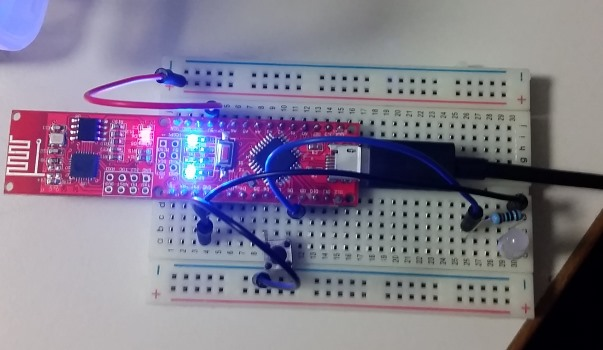
\includegraphics[scale=0.6]{Pretzel_Projekt.jpg}
	\caption[Pretzelboard im Projekt]{Pretzelboard im Projekt,\\ Quelle: Eigene Aufnahme}
\end{figure}

%Bild vom fertigen Button
\newpage

\subsection{ESP8266 Lua}
\label{sec:ESP8266}

\subsubsection{Vorstellung des ESP8266 Lua}        
\label{sec:Vorstellung des ESP8266} 

Der ESP8266 Lua ist ein Entwicklungsboard, welches bereits ein integriertes WLAN Modul besitzt und mit einem \ac{TCP}/\ac{IP} Stack ausgestattet ist. Einer der vorgesehenen Einsatzzwecke ist unter anderem das Internet of Things. Das Board kann zudem mit Steckbrett arbeiten und bietet daher ähnliche Möglichkeiten, wie das bereits erwähnte \nameref{sec:Pretzelboard-1}. Zudem ist es möglich, dass die Software für das ESP8266 Lua Entwicklungsboard ebenfalls über die Arduino \ac{IDE} entwickelt werden kann. Allerdings sind technische Unterschiede zum Pretzelboard vorhanden, was dazu führt, dass andere Treiber genutzt werden müssen. 
Diese können nachinstalliert werden und stehen dann zur Nutzung des Boards bereit. (vgl. \cite{Carius.15.01.2017}\cite{.d})

\begin{figure}[!htb]
	\centering
	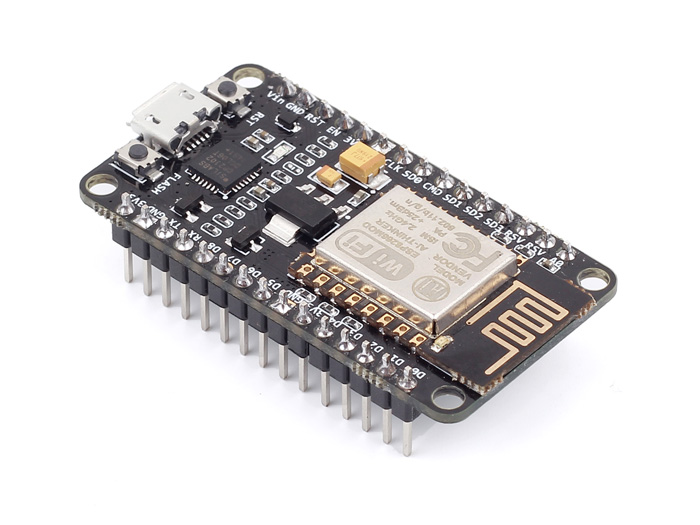
\includegraphics[scale=0.4]{ESP.jpg}
	\caption[ESP8266]{ESP8266,\\ Quelle: https://www.roboter-bausatz.de/media/image/dc/14/6e/113990105-1.jpg}
\end{figure}

\subsubsection{Verwendung im Projekt}        
\label{sec:Verwendung des ESP8266} 
Das Board wird im Rahmen des Projektes als weiterer Button genutzt. Es bietet sich für diese Funktion an, da es ebenfalls recht klein ist und alle benötigten Funktionen bereits vorhanden sind. Neben den vorhandenen Funktionen ist auch die Möglichkeit vorhanden, dass eine bereits durch das Pretzelboard bekannte Entwicklungsumgebung genutzt werden kann. Das bietet die Möglichkeit, dass statt des \ac{UDP} Protokolls das bereits erwähnte \nameref{sec:TCP-1} Protokoll ausprobiert werden kann. 
Der Aufbau des Boards soll ebenfalls durch ein Elektroniksteckboard umgesetzt werden. Dazu wird das Board auf eben dieses Steckboard gesetzt und mit einem Button, Statusleuchten und entsprechenden Kabeln verbunden. Nach der Betätigung des Buttons wird das Board geweckt und eine Funktion schickt ein entsprechendes Datenpaket an einen Empfänger.
\begin{figure}[!htb]
	\centering
	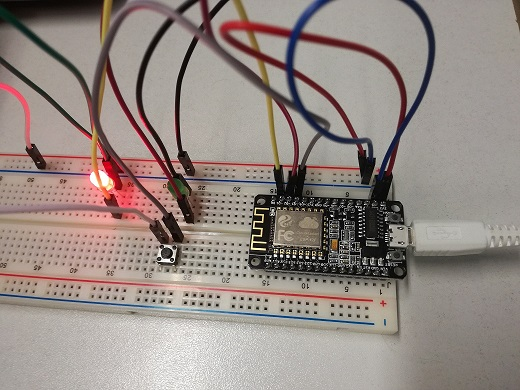
\includegraphics[scale=0.5]{ESP_Projekt.jpg}
	\caption[ESP8266 im Projekt]{ESP8266 im Projekt,\\ Quelle: Eigene Aufnahme}
\end{figure}
\newpage


 

%Bild vom fertigen Button 

\subsection{Amazon Dash Button}
\label{sec:Amazon Dash Button}

\subsubsection{Vorstellung des Amazon Dash Buttons}        
\label{sec:Vorstellung des Amazon Dash Buttons} 
Am 31.08.16 wurde der Amazon Dash Button offiziell in Deutschland exklusiv für Prime Mitglieder eingeführt (vgl. \cite{ONLINE.31.08.2016}).
Dabei handelt es sich um einem mit dem WLAN verbundenen Button, mit welchem sich zum Großteil Verbrauchsartikel per Knopfdruck bestellen lassen.
Jeder Button wird mit einem Produkt verknüpft, das während des Einrichtens ausgewählt wird.
Sollte nun das Produkt zur Neige gehen oder gar aufgebraucht sein, so kann der Nutzer den Button drücken und es wird sofort ein Bestellvorgang eingeleitet.
Weitere Interaktion seitens des Nutzers ist dabei nicht notwendig.

Der Dash Button wird über die Amazon App auf einem Android- oder iOS-Smartphone eingerichtet und verwaltet und funktioniert an allen Orten mit einer WLAN-Verbindung.
Sobald die Einrichtung abgeschlossen ist, wird eine Benachrichtigung (sofern aktiviert) an das Smartphone versendet, immer wenn eine Bestellung aufgegeben wurde (vgl. \cite{.dash}).
Zusätzlich verfügt der Button über einen Bestellschutz.
Mit dieser Funktion gibt der Dash Button keine Bestellung auf, bis die vorherige Bestellung geliefert wurde – egal wie oft der Dash Button gedrückt wird.
Der Amazon Dash Button ist in Deutschland für aktuell 4,99  \euro  erhältlich (Stand: 17.05.17).
Jedoch wird dieser Preis mit der ersten Bestellung verrechnet, wodurch dem Kunden keine zusätzlichen Kosten entstehen.

\begin{figure}[!htb]
	\centering
	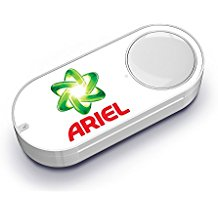
\includegraphics[scale=0.5]{Dash.jpg}
	\caption[Amazon Dash Button für Produkte von Ariel]{Amazon Dash Button für Produkte von Ariel,\\ Quelle: https://images-eu.ssl-images-amazon.com/images/I/41SMHhklQYL.\_A
	C\_US218\_.jpg}
\end{figure}

\subsubsection{Untersuchung des Amazon Dash Buttons}
\label{sec:Untersuchung des Amazon Dash Buttons}
Die Untersuchung des Amazon Dash Buttons bezieht sich nur auf dessen Funktionen.
Die Hardware wurde nicht analysiert, da diese bereits mehrfach, auch auf unterschiedlichen Websites analysiert wurde (vgl. \cite{.17.05.2017}\cite{.17.05.2017b}).

Der Amazon Dash Button wird einem kleinen braunen Karton geliefert.
Dieser enthält neben dem Button noch 2 Dokumente, eine Gebrauchsanleitung und Sicherheitsinformationen.
Die Gebrauchsanleitung beschreibt nur den Download der Amazon App sowie die schritte, die notwendig sind um den Konfigurationsassistenten zu starten.

Die eigentlich Einrichtung läuft dann wie folgt ab:
Zuerst müssen WLAN und Bluetooth auf dem Gerät aktiviert werden.
Danach muss der Amazon Dash Button für ca. 6 Sekunden gedrückt werden, bis dieser Blau leuchtet.
Dann muss der Benutzer auf seinem Smartphone auf "`Verbinden"' drücken.
Die Amazon App versucht sich dann via Bluetooth mit dem Button zu verbinden.
Sollte dies erfolgreich sein, so kann der User das  Produkt auswählen, welche auf dem Button hinterlegt werden soll.

Hierbei hat der Benutzer hier nur auf eine sehr kleine Auswahl des Herstellers Zugriff.
So gibt es beispielsweise bei dem "`Power Point Energy Drink Dash Button"' nur eine Auswahl aus 4 Produkten:
\begin{itemize}
\item Power Point Energy Drink Classic, 24er Pack (24 x 250 ml)
\item Power Point Energy Drink Himbeere, 24er Pack (24 x 250 ml)
\item Power Point Energy Drink Waldmeister, 24er Pack (24 x 250 ml)
\item Power Point Energy Drink Ice Blue , 24er Pack (24 x 250 ml) 
\end{itemize}
Hat der Benutzer seine Auswahl getroffen, muss er noch den Dash Button mit einem WLAN Netzwerk verbinden.
Dabei sucht der Dash Button nach verfügbaren Netzwerken welche dann dem Benutzer in der Amazon App angezeigt werden.
Nun muss der Benutzer nur noch ein WLAN Netzwerk auswählen, das Passwort für dieses eingeben und schon kann der Button benutzt werden.

\subsubsection{Verwendung des Amazon Dash Buttons im Projekt}
\label{sec:Verwendung des Amazon Dash Buttons im Projekt}
Der Amazon Dash Button konnte erfolgreich in das Projekt eingebunden werden. Hierbei waren jedoch ein paar Workarounds notwendig, welche in \ref{sec:Einbindung des Amazon Dash Buttons-1} näher ausgeführt werden. Dabei funktioniert der Dash Button genauso wie die selbst einwickelten Button.
%Bild vom Button 
\newpage

\section{Umsetzung des Projektes}        
\label{sec:Umsetzung des Projektes-1}  


\subsection{Architektur und Zusammenarbeit der Komponenten}        
\label{sec:Architektur und Zusammenarbeit der Komponenten-1} 

Mithilfe der Technologien und Softwarelösungen, die in Kapitel \ref{sec:Theorie-1} erläutert worden sind, und der Hardware, die in Kapitel \ref{sec:Beschreibung der Hardware-1} vorgestellt wurde, konnten die verschiedenen Komponenten, die bereits in der Aufgabenstellung (vgl. Kapitel \ref{sec:Aufgabenstellung-1}) genannt worden sind, umgesetzt werden. 
Im folgenden soll ein Überblick über die Zusammenarbeit der einzelnen Komponenten gegeben werden, bevor in den folgenden Kapiteln auf die genaue Entwicklung der einzelnen Komponenten eingegangen wird. 

Für den Nutzer gibt es ein Webfrontend, welches mithilfe eines Nginx Webservers (vgl. Kapitel {sec:WebserverNginx-1}) realisiert wird. Dieses Webfrontend greift auf ein \ac{REST} \ac{API}-Backend zurück, welches in \ac{PHP} geschrieben wurde und ebenfalls über den Nginx realisiert wird. Mithilfe dieses Backends werden die verschiedenen \ac{API} Routen realisiert, die dann den Zugriff auf die Datenbank organisieren. Das Backend besteht ebenfalls aus einigen Skripten, die in Python\ref{src:Python-1}) geschrieben sind. Diese Skripte organisieren die Kommunikationsendpunkte für die Buttons, indem sie auf die entsprechende Kommunikationsports für die Datenpakete lauschen und die Daten dann verarbeiten. 

Neben der Kommunikation wird ebenfalls ein Teil der \ac{REST} \ac{API} in Python realisiert. Dieser Teil ermöglicht sowohl den Status der Skripte, die die Kommunikation organisieren, abzufragen als auch die Skripte neu zu starten, sollte ein Skript nicht gestartet sein oder ein Fehler aufgetreten sein. Diese Daten werden ebenfalls für das Webfrontend verwendet. 
Die Buttons, als weitere Komponente, werden durch verschiedene Hardwareelemente realisiert. Mithilfe entsprechender Programme, die auf die Controller geladen werden, stellen sie eine Verbindung zu den definierten Kommunikationspunkten her. Über dieses Kommunikationsprotokoll werden dann, sobald der Button betätigt wurde, die entsprechenden Daten gesendet und dann im Backend verarbeitet. 
Zur Verarbeitung der Daten gehört auch das Einfügen in die entsprechenden Tabellen der SQL Datenbank, die auf einem MySQL Datenbankserver läuft, der für die Verwaltung der Daten zuständig ist. 
% Vielleicht noch ein passendes Modell einfügen


\newpage

\subsection{Entwicklung der Buttons}  
\label{sec:Entwicklung der Buttons-1} 

Im folgenden soll auf die Entwicklung der Button Komponente im Projekt eingegangen werden. Dabei wird insbesondere auf die Programmierung und Umsetzung eingegangen werden. 
Bei der Entwicklung der verschiedenen Buttons wurde insbesondere darauf geachtet, dass verschiedene Technologien getestet werden, um möglichst viele technische Möglichkeiten zu untersuchen. Das ist damit zu begründen, dass das Untersuchen von möglichst vielen Möglichkeiten zum Projektziel gehörte. 

\subsubsection{Entwicklung mit dem ``Pretzelboards''}  
\label{sec:Entwicklung mit dem ``Pretzelboards''-1}

\subsubsection{Entwicklung mit dem ESP8266 Lua}  
\label{sec:Entwicklung mit dem ESP8266-1}

\subsubsection{Einbindung des Amazon Dash Buttons}  
\label{sec:Einbindung des Amazon Dash Buttons-1}
% bitte hier einbinden, dass es mithilfe eines entsprechenden Pythonscript und ifabfragen auf die MAC Adresse möglich wäre, dass man diese Buttons wirklich einsetzen könnte (stimmt doch?) 

\newpage

\subsection{Entwicklung des Frontends}  
\label{sec:Entwicklung der Frontends-1} 

\subsubsection{Aufbau und Entwicklung des Frontends}  
\label{sec:Aufbau und Entwicklung des Frontends-1}

\newpage

\subsection{Entwicklung und Einrichtung des Backends}  
\label{sec:Entwicklung und Einrichtung des Backends-1} 

In den folgenden Kapiteln wird auf die Einrichtung des Backends eingegangen. Dies umfasst sowohl die Einrichtung des Raspberry Pis, den Aufbau und die Entwicklung der REST API und die Entwicklung der Python Skripte. Die Einrichtung des Raspberry PIs wird an dieser Stelle geführt, da er das zentrale Hardwareelemente im Backend ist, da er genutzt wird, um die entsprechende Softwaredienste zur Verfügung zu stellen. Er stellt den zentralen Kommunikationspunkt im Projekt dar, da die Buttons nur ihn kennen, sich aber nicht gegenseitig. 

\subsubsection{Einrichtung des Raspberrys}  
\label{sec:Einrichtung des Raspberrys-1}

Die Einrichtung des Raspberry PIs besteht aus mehreren Schritten an dessen Ende die Verwendung des Raspberrys als zentraler Server steht. Die verschiedenen Schritte werden im folgenden erklärt: 
\paragraph{Einrichtung des Nginx}  
\label{sec:Einrichtung des Nginx-1} 

\paragraph{Einrichtung des SQL Datenbankservers}  
\label{sec:Einrichtung des SQL Datenbankservers-1} 

\paragraph{Einrichtung des WLAN Access Points}  
\label{sec:Einrichtung des WLAN Access Points-1} 

\paragraph{Einrichtung des UDP Empfängers}  
\label{sec:Einrichtung des UDP Empfängers-1} 

\paragraph{Einrichtung des TCP Empfängers}  
\label{sec:Einrichtung des TCP Empfängers-1} 


\subsubsection{Aufbau und Entwicklung der Python Skripte}  
\label{sec:Aufbau und Entwicklung der Python Skripte-1}

Mithilfe der Skriptsprache Python werden die verschiedenen Kommunikationsendpunkte in Form von Sockets realisiert. Um eine bessere Übersichtlichkeit zu gewährleisten und eine zentrale Verwaltung zu haben, gibt es ein Verwaltungsskript. Dieses Skript startet die anderen Skripte, die sich um jeweils einen Kommunikationsprotokoll kümmern. So gibt es ein Skript für die Kommunikation über \ac{UDP}, eins für \ac{TCP} und eins für \ac{ARP}, welches für die Amazon Dash Buttons genutzt wird. Aus diesen Gründen gibt es insgesamt vier Python Skripte, die einen wesentlichen Teil des Backends ausmachen.

\paragraph{Entwicklung des Verwaltungsskripts}$\;$ \\  
\label{sec:Entwicklung des Verwaltungsskripts-1} 
Das Verwaltungsskript dient, wie bereits erwähnt, als zentrales Skript, welches als einziges Skript auch gestartet werden muss. Über dieses Skript werden dann alle anderen notwendigen Skripte gestartet, die dann dafür sorgen, dass die Kommunikation ermöglicht wird. 
Neben dieser Funktionalität wird durch das Verwaltungsskript auch eine \ac{REST} \ac{API} realisiert. Diese wird mithilfe des Frameworks Flask (vgl. \cite{.s}) umgesetzt. Diese \ac{API} wird dazu genutzt, um einige Funktionalitäten bereitzustellen, die im Frontend benötigt werden. Als Beispiel wäre der aktuelle Status der Empfängerskripte (vgl. Kapitel \ref{sec:Entwicklung des UDP Skripts-1}) zu nennen. 

Die genannte \ac{REST} \ac{API} kann dann im Verwaltungsskript auf andere Methoden zugegriffen werden, die dann weitere Funktionen umfassen. Die Rückgabewerte dieser Funktionen werden dann im \ac{JSON} Format an das Frontend der Anwendung weitergegeben und können dann dort weiter verarbeitet werden. So kann beispielsweise im Frontend angezeigt werden, dass alle Kommunikationsmöglichkeiten zur Verfügung stehen. 

\paragraph{Entwicklung des \ac{UDP} Skripts}$\;$ \\  
\label{sec:Entwicklung des UDP Skripts-1} 
Da die Übertragung der Datenpakete über das \ac{UDP} Protokoll ermöglicht werden soll, muss ein entsprechender Empfänger auf dem Raspberry PI vorhanden sein. Dieser Empfänger wird mithilfe eines Skriptes in Python realisiert.

Dieses Skript nutzt die Library ``Socket'' (vgl. \cite{.20.02.2017}), welches es ermöglicht ein Socket zu erstellen. Dieses Socket wird an eine \ac{IP} Adresse und einen Port gebunden und wird anschließend für alle eingehenden \ac{UDP} Pakete genutzt. In einer Endlosschleife, welche manuell unterbrochen werden kann, wird auf eingehende Pakete gewartet. Die Endlosschleife wird benötigt, da ein Button zu jedem Zeitpunkt betätigt werden kann und somit dauerhaft auf ankommende Pakete geachtet werden muss. 

Bei Eingang eines entsprechenden Pakets wird ein entsprechendes Request an die \ac{REST} \ac{API} geschickt. Da als Übertragungsart allerdings das \ac{UDP} Protokoll genutzt wird, kann dem Button keine Rückmeldung gegeben werden, ob der Eintrag in die Datenbank über die \ac{REST} \ac{API} erfolgreich war. Zudem kann auch kein allgemeines Feedback zurückgegeben werden. Auch bei anderen Fehlern kann dem Button keine Rückmeldung gegeben werden. 

Nach dem erfolgreichen Absenden der Anfrage an die \ac{REST} \ac{API} befindet sich das Skript für den \ac{UDP} Empfänger weiterhin in der Endlosschleife und wartet auf das nächste Datenpaket. 
Das Skript ist im Anhang unter \ref{sec:UDPAnhang} zu finden. 

\paragraph{Entwicklung des \ac{TCP} Skripts}$\;$ \\  
\label{sec:Entwicklung des TCP Skripts-1} 
Für alle Datenpakete, die über das Protokoll \ac{TCP} empfangen werden, muss ebenfalls ein Skript geschrieben werden, welches diese Datenpakete verarbeitet. Dabei wird genauso vorgegangen, wie beim Skript für \ac{UDP}. Der einzige Unterschied ist nach dem Absenden der Anfrage an die \ac{REST} \ac{API}. Das Skript für \ac{TCP} Datenpakete wartet nach dem Absenden der Anfrage auf die Bestätigung und schickt eine entsprechende Antwort zurück an den Button. Dieser verarbeitet ebenfalls die Antwort und kann mithilfe einer Lampe auf dem Steckbrett dem Nutzer ein visuelles Feedback geben. 
Das entsprechende Skript ist im Anhang unter \ref{sec:TCPAnhang} zu finden.

\paragraph{Entwicklung des \ac{ARP} Skripts}$\;$ \\  
\label{sec:Entwicklung des ARP Skripts-1} 
Da das Mitlesen der \ac{IP} Datenpakete des Amazon Dash Buttons nicht möglich war, wurde das mitschneiden der \ac{ARP} Datenpakete notwendig, wie bereits in Kapitel \ref{sec:Einbindung des Amazon Dash Buttons-1} beschrieben. 
Im Vergleich zu den Skripten, die in den Kapiteln \nameref{sec:Entwicklung des UDP Skripts-1} und \nameref{sec:Entwicklung des TCP Skripts-1} beschrieben sind, ist dieses Skript etwas anders aufgebaut. Es wird zwar ebenfalls die Library ``Socket'' genutzt, allerdings ist die Konfiguration des Sockets anders, damit \ac{ARP} Datenpakete gelesen werden können. 


Das Lesen dieser Datenpakete beschränkt sich allerdings auf das Erkennen der \ac{IP} Adresse, die das Paket abschickt bzw. empfängt. Nur diese Informationen werden benötigt, da die Funktionalität des Skript darauf beruht, dass jeder zweite \ac{ARP} Request eine entsprechende Anfrage an die \ac{REST} \ac{API} abschickt. Das nur jeder zweite Request eine entsprechende Anfrage abschickt, ist damit begründet, dass bei einem einzelnen Druck auf den Amazon Dash Button ein \ac{ARP} Paket von Button zum Router geschickt wird und ein Paket vom Router zum Button. Das bedeutet, dass für jeden Druck zwei Requests abgeschickt werden. Daher löst nur jedes zweite Paket eine Anfrage aus, die dann die Anzahl eines Produktes in der Datenbank erhöht. 

Dies wird durch einen entsprechenden Zähler im Skript umgesetzt, welcher bei eins startet und bei dem Wert zwei eine entsprechende Anfrage an die \ac{REST} \ac{API} abschickt. Nach dem Abschicken der Anfrage wird der Zähler wieder auf eins gesetzt. 
Durch eine Unterscheidung von \ac{MAC} Adressen, welche ebenfalls im \ac{ARP} Header mitgeschickt werden, ist es auch möglich, dass verschiedene Amazon Dash Buttons eingebunden werden. 
Allerdings benötigt diese Konfiguration einige manuelle Arbeit, da das Skript nur manuell zu bearbeiten ist. 
Das entsprechende Skript ist im Anhang unter \ref{sec:ARPAnhang} zu finden.

\newpage

\section{Ergebnis des Projektes}        
\label{sec:Ergebnis des Projektes-1}  

\section{Fazit und Ausblick}        
\label{sec:Fazit und Ausblick-1}  

\newpage
\addcontentsline{toc}{section}{Literaturverzeichnis}
\bibliographystyle{unsrt}  
\bibliography{Literatur}

\section*{Anhang}   
\addcontentsline{toc}{section}{Anhang}     
\label{sec:Anhang-1}  

\subsection*{Skripte}  
\label{sec:Skripte-1} 

\subsubsection*{Python Skripte}
\label{sec:Pythonskripte}

Alle Python Skripte, die verwendet wurden: 

\paragraph{UDP Skript für den Raspberry PI:}$\;$ \\  
\lstinputlisting[language=Python]{textteile/udp.py}
\newpage

\paragraph{TCP Skript für den Raspberry PI:}$\;$ \\  
\lstinputlisting[language=Python]{textteile/tcp.py}
\newpage

\paragraph{ARP Skript für den Raspberry PI:}$\;$ \\  
\lstinputlisting[language=Python]{textteile/amazon.py}
\newpage

\paragraph{Service Skript für den Raspberry PI:}$\;$ \\  
\lstinputlisting[language=Python]{textteile/service.py}
\newpage

\subsubsection*{MySQL Skript}
\label{sec:MySQLSkript}
Das Skript zur Einrichtung der Datenbank
\lstinputlisting[language=Python]{textteile/mysqlscript.txt}

\subsection*{Konfigurationsdateien}  
\label{sec:Konfigurationsdateien-1} 

\subsubsection*{Nginx Konfiguration}
\label{sec:NginxKonfiguration}
Die Konfigurationsdatei des Nginx Webservers. 
\lstinputlisting[language=Python]{textteile/nginxconfig.txt}


\subsubsection*{Hostapd Konfiguration}
\label{sec:HostapdSkript}
Die Konfigurationsdatei von hostapd
\lstinputlisting[language=Python]{textteile/hostapdconf.txt}

\subsubsection*{Interfaces Konfiguration}
\label{sec:NginxSkript}
Die Konfigurationsdatei ``interfaces''
\lstinputlisting[language=Python]{textteile/interfaces.txt}



\end{document}